\chapter{Results}


\begin{table}[h]
	\resizebox{\textwidth}{!}{%
	\begin{tabular}{llllrrrrrrrrr}
	\toprule
% 	 &  &  &  & \rotatebox{70}{\textbf{k_r2r_d}} & \rotatebox{70}{\textbf{k_r2r_min}} & \rotatebox{70}{\textbf{k_dig}} & \rotatebox{70}{\textbf{k_r2r+_d}} & \rotatebox{70}{\textbf{k_r2r+_min}} & \rotatebox{70}{\textbf{k_r2r+_max}} & \rotatebox{70}{\textbf{k_dig+_2}} & \rotatebox{70}{\textbf{k_c2r+}} & \rotatebox{70}{\textbf{mean}} \\
	\textbf{Preprocessing} & \specialcell[b]{\textbf{Quanti-}\\ \textbf{fication}} & \textbf{\#Dims} & \specialcell[b]{\textbf{Doc-Term-}\\ \textbf{Matrix} \\ \textbf{Quanti-}\\ \textbf{fication}} & \rotatebox{70}{\textbf{k_r2r_d}} & \rotatebox{70}{\textbf{k_r2r_min}} & \rotatebox{70}{\textbf{k_dig}} & \rotatebox{70}{\textbf{k_r2r+_d}} & \rotatebox{70}{\textbf{k_r2r+_min}} & \rotatebox{70}{\textbf{k_r2r+_max}} & \rotatebox{70}{\textbf{k_dig+_2}} & \rotatebox{70}{\textbf{k_c2r+}} & \rotatebox{70}{\textbf{mean}} \\
	\midrule
	\multirow[t]{24}{*}{\mfauhcsdT} & \multirow[t]{8}{*}{\textbf{count}} & \multirow[t]{2}{*}{\textbf{3}} & \textbf{ppmi} & 0 & 1 & 0 & 145 & 370 & 510 & 191 & - & 174 \\
	 &  &  & \textbf{tfidf} & 0 & 1 & 0 & 110 & 237 & 278 & 83 & - & 101 \\
	\cline{3-4}
	 &  & \multirow[t]{3}{*}{\textbf{100}} & \textbf{count} & 0 & 5 & 0 & 0 & 114 & 52 & 290 & 0 & 58 \\
	 &  &  & \textbf{ppmi} & 0 & 6 & 27 & 139 & 224 & 247 & 120 & - & 109 \\
	 &  &  & \textbf{tfidf} & 0 & 6 & 5 & 246 & 270 & 281 & 201 & - & 144 \\
	\cline{3-4}
	 &  & \multirow[t]{3}{*}{\textbf{200}} & \textbf{count} & 0 & 5 & 1 & 0 & 133 & 52 & 509 & 0 & 88 \\
	 &  &  & \textbf{ppmi} & 0 & 6 & 57 & 196 & 315 & 344 & 90 & - & 144 \\
	 &  &  & \textbf{tfidf} & 0 & 6 & 17 & 357 & 370 & 372 & 433 & - & 222 \\
	\cline{2-4} \cline{3-4}
	 & \multirow[t]{8}{*}{\textbf{ppmi}} & \multirow[t]{2}{*}{\textbf{3}} & \textbf{ppmi} & 0 & 0 & 0 & 192 & 247 & 363 & 136 & - & 134 \\
	 &  &  & \textbf{tfidf} & 0 & 0 & 0 & 169 & 206 & 217 & 59 & - & 93 \\
	\cline{3-4}
	 &  & \multirow[t]{3}{*}{\textbf{100}} & \textbf{count} & 0 & 0 & 0 & 0 & 38 & 25 & 242 & 0 & 38 \\
	 &  &  & \textbf{ppmi} & 0 & 0 & 0 & 80 & 112 & 101 & 22 & - & 45 \\
	 &  &  & \textbf{tfidf} & 0 & 0 & 0 & 89 & 90 & 96 & 85 & - & 51 \\
	\cline{3-4}
	 &  & \multirow[t]{3}{*}{\textbf{200}} & \textbf{count} & 0 & 0 & 0 & 0 & 34 & 21 & 293 & 0 & 44 \\
	 &  &  & \textbf{ppmi} & 0 & 1 & 112 & 100 & 163 & 163 & 37 & - & 82 \\
	 &  &  & \textbf{tfidf} & 0 & 1 & {\cellcolor{lightgreen}} 127 & 99 & 107 & 106 & 131 & - & 82 \\
	\cline{2-4} \cline{3-4}
	 & \multirow[t]{8}{*}{\textbf{tfidf}} & \multirow[t]{2}{*}{\textbf{3}} & \textbf{ppmi} & 0 & 0 & 0 & 229 & 357 & 423 & 84 & - & 156 \\
	 &  &  & \textbf{tfidf} & 0 & 0 & 0 & 169 & 255 & 258 & 24 & - & 101 \\
	\cline{3-4}
	 &  & \multirow[t]{3}{*}{\textbf{100}} & \textbf{count} & 0 & 1 & 0 & 0 & 162 & 64 & 450 & 0 & 85 \\
	 &  &  & \textbf{ppmi} & 0 & 1 & 3 & 324 & 404 & 423 & 151 & - & 187 \\
	 &  &  & \textbf{tfidf} & 0 & 1 & 0 & 390 & 422 & 437 & 425 & - & 239 \\
	\cline{3-4}
	 &  & \multirow[t]{3}{*}{\textbf{200}} & \textbf{count} & 0 & 2 & 0 & 0 & 211 & 83 & {\cellcolor{lightgreen}} 869 & {\cellcolor{lightgreen}} 1 & 146 \\
	 &  &  & \textbf{ppmi} & 0 & 2 & 13 & 395 & {\cellcolor{lightgreen}} 559 & {\cellcolor{lightgreen}} 577 & 153 & - & 243 \\
	 &  &  & \textbf{tfidf} & 0 & 2 & 0 & {\cellcolor{lightgreen}} 531 & 554 & 572 & 794 & - & {\cellcolor{lightgreen}} 350 \\
	\cline{1-4} \cline{2-4} \cline{3-4}
	\multirow[t]{24}{*}{\mfauhtcsldp} & \multirow[t]{8}{*}{\textbf{count}} & \multirow[t]{2}{*}{\textbf{3}} & \textbf{ppmi} & 0 & 1 & 0 & 226 & 319 & 317 & 208 & - & 153 \\
	 &  &  & \textbf{tfidf} & 0 & 1 & 0 & 210 & 214 & 215 & 82 & - & 103 \\
	\cline{3-4}
	 &  & \multirow[t]{3}{*}{\textbf{100}} & \textbf{count} & 0 & 7 & 0 & 0 & 118 & 61 & 230 & 0 & 52 \\
	 &  &  & \textbf{ppmi} & 0 & 8 & 27 & 184 & 256 & 262 & 125 & - & 123 \\
	 &  &  & \textbf{tfidf} & 0 & 8 & 5 & 253 & 255 & 255 & 168 & - & 135 \\
	\cline{3-4}
	 &  & \multirow[t]{3}{*}{\textbf{200}} & \textbf{count} & 0 & 8 & 0 & 0 & 117 & 64 & 290 & 0 & 60 \\
	 &  &  & \textbf{ppmi} & 0 & {\cellcolor{lightgreen}} 11 & 41 & 200 & 319 & 325 & 88 & - & 141 \\
	 &  &  & \textbf{tfidf} & 0 & {\cellcolor{lightgreen}} 11 & 8 & 331 & 333 & 333 & 302 & - & 188 \\
	\cline{2-4} \cline{3-4}
	 & \multirow[t]{8}{*}{\textbf{ppmi}} & \multirow[t]{2}{*}{\textbf{3}} & \textbf{ppmi} & 0 & 0 & 0 & 138 & 310 & 321 & 254 & - & 146 \\
	 &  &  & \textbf{tfidf} & 0 & 0 & 0 & 143 & 148 & 150 & 187 & - & 90 \\
	\cline{3-4}
	 &  & \multirow[t]{3}{*}{\textbf{100}} & \textbf{count} & 0 & 0 & 0 & 0 & 29 & 11 & 186 & 0 & 28 \\
	 &  &  & \textbf{ppmi} & 0 & 1 & 0 & 117 & 142 & 142 & 20 & - & 60 \\
	 &  &  & \textbf{tfidf} & 0 & 1 & 0 & 122 & 124 & 124 & 103 & - & 68 \\
	\cline{3-4}
	 &  & \multirow[t]{3}{*}{\textbf{200}} & \textbf{count} & 0 & 1 & 0 & 0 & 25 & 10 & 272 & 0 & 38 \\
	 &  &  & \textbf{ppmi} & 0 & 1 & 48 & 126 & 161 & 165 & 28 & - & 76 \\
	 &  &  & \textbf{tfidf} & 0 & 1 & 17 & 143 & 144 & 148 & 133 & - & 84 \\
	\cline{2-4} \cline{3-4}
	 & \multirow[t]{8}{*}{\textbf{tfidf}} & \multirow[t]{2}{*}{\textbf{3}} & \textbf{ppmi} & 0 & 0 & 0 & 146 & 219 & 223 & 133 & - & 103 \\
	 &  &  & \textbf{tfidf} & 0 & 0 & 0 & 108 & 111 & 109 & 38 & - & 52 \\
	\cline{3-4}
	 &  & \multirow[t]{3}{*}{\textbf{100}} & \textbf{count} & 0 & 1 & 0 & 0 & 160 & 54 & 389 & 0 & 76 \\
	 &  &  & \textbf{ppmi} & 0 & 2 & 9 & 281 & 375 & 380 & 205 & - & 179 \\
	 &  &  & \textbf{tfidf} & 0 & 2 & 0 & 373 & 377 & 392 & 339 & - & 212 \\
	\cline{3-4}
	 &  & \multirow[t]{3}{*}{\textbf{200}} & \textbf{count} & 0 & 3 & 0 & 0 & 199 & 64 & 661 & 0 & 116 \\
	 &  &  & \textbf{ppmi} & 0 & 3 & 21 & 362 & 456 & 472 & 164 & - & 211 \\
	 &  &  & \textbf{tfidf} & 0 & 3 & 1 & 499 & 498 & 501 & 645 & - & 307 \\
	\bottomrule
	\end{tabular}
	}
	\caption{Number of Candidate-Phrases for different parameter-combinations and kappa-values \label{tab:kappa_table}}
	\label{tab:cands_per_config}
\end{table}

	
		
\section{Evaluation} %TODO what is this for a title? it sucks

\begin{itemize}
	\item \cite{Derrac2015} evaluated using a bunch of commonsense reasoning based classifiers (want to show that at least as performant than standard approaches, but can give intuitive explanations) (these reasoning-classifiers can be linked to intuitive explanations: 1-NN is "Y is of the same class as X because X closest to Y", but also more complex ones.) 
	\item 
\end{itemize}

* This is clustering and looking if it corresponds to human judgement, which unfortunately doesn't allow for a simple accuracy and be done with it.
* So, the papers that did this come up with a few things
* [TODO: the shallow decisiontrees of one of the followups]
* DESC15 "evaluate the practical usefulness of the considered semantic relations" by checking "their use in commonsense reasoning based classifiers", like interpolation and a fortiori inference (chap 5)


* DESC15 tests like this: Section 6.1: Evaluate whether the derived relations are sufficiently accurate for classification, and 6.2 is then comparison with crowdsourcing experiments (more subjective aspects, the question “are the relations useful explanations?”)



\section{Qualitative Analysis}

Qualitative Analysis in this case means "looking at stuff". Such a qualitative analysis is always to be taken with a grain of salt, because it is very prone to cherry-picking (both on purpose and not on purpose, the stuff you're looking at just doesn't need to be representative!). However it does help a lot and provides a lot of insights (and often helped me in the debugging process).
What can you look at for such a qualitative analysis?
\begin{itemize}
	\item The clusters, checking if things you know to be similar are actually in the same clusters
	\item If descriptions you know to be semantically similar are actually close in the embedding
	\item You can do the whole thing for only three dimensions instead of the 50/100/200 because there you can plot the stuff and interpret it
\end{itemize}

\begin{itemize}
	\item  Man kann ja schon nach dem Embedding anhand der nächsten Entities sehen ob das was werden kann - bei 100D sind dann halt "airplane cabin" und "aircraft cabin" die nächsten entities, bei 3D dann halt eher kram wie "area" and "moor", was schon eindeutig zeigt dass 3D offensichtlich nicht so der Hit ist
	\item Die vielen Sanity Checks die man machen kann, bspw dass ich ja in 3D gucken kann (und auch in höher-D ausrechnen) ob eben diese dinge (von item 1) im Embedding nah sind, und ob die SVM Dinge schön trennt ("howto_embed.ipynb")
	\item "placetypes_origconf.ipynb", was einfach von vorne bis hinten die original-config (ist ja auch im yaml) von DESC15 ausführt und interpretiert	
\end{itemize}

\begin{figure}[H]
	\centering
	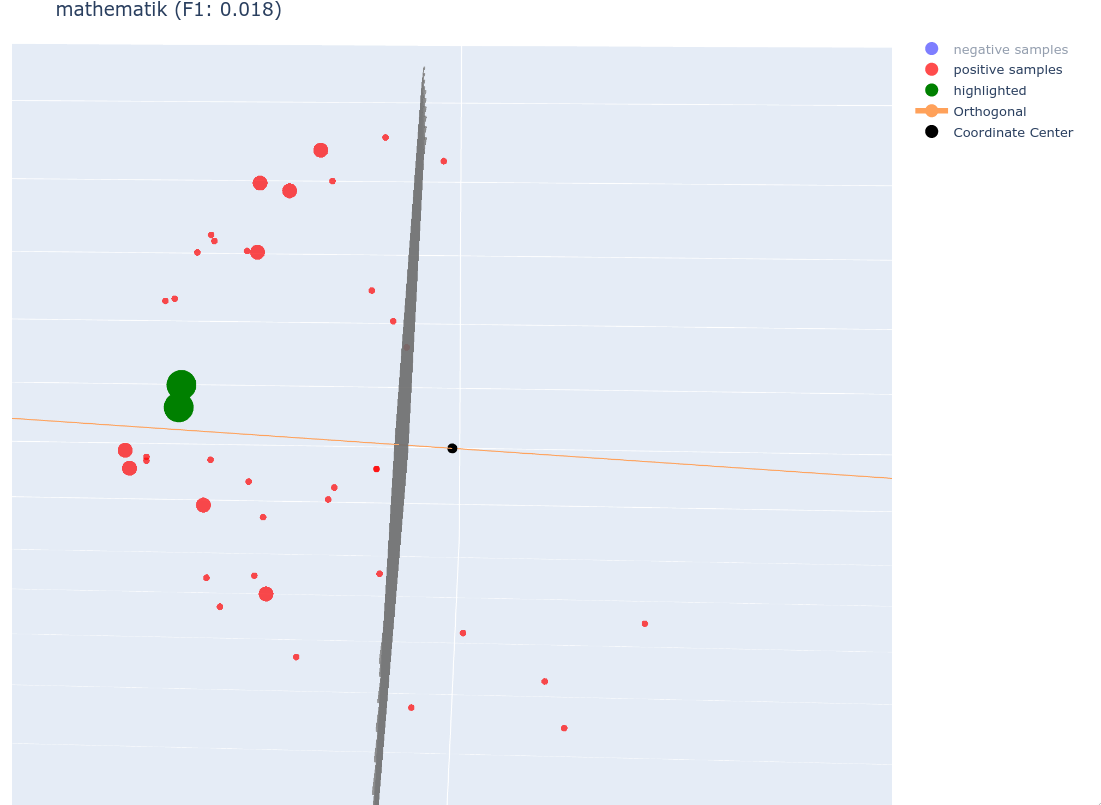
\includegraphics[width=\figwidth]{svm_mathematik_highlight_infoAB.png}
	\caption[3D-Plot with an SVM for the term "Mathematik"]{
		\label{fig:3dplot_mathe_infoab}
		3D-Plot with an SVM for the term "Mathematik", also highlighting the courses "Informatik A" and "Informatik B"
	}
\end{figure}

In figure \ref{fig:3dplot_mathe_infoab} we see a 3D-Embedding for courses, splitting courses which contain the term "mathematics" from those that don't, also hightlighting the terms "Informatik A" and "Informatik B". We see they are close we see the SVM is not to bad, and even though neiher Info A nor Info B contains the word "mathematik", thy are both on the "mathematical side" of courses. Negative samples are hidden for better visibility, and entities that contain the word more-often-than-the 75th (???) percentile have bigger markers.


\begin{itemize}
	\item In 3D ists immer ne Kugel, und ich würde behaupten in höheren Dimensionen ist es nicht extrem viel besser. dadrin ne SVM zu machen bringt echt wenig bis gar nix (Ich hab ja sogar Plots die zeigen dass die Movies viel besser clustern - TODO: die einbringen)
\end{itemize}


\section{Quantiative Results}

% Schreiben was die paper denen ich mostly folge zur evaluation gemacht haben! ("To evaluate whether the discovered features are semantically meaningful, we test how similar they are to natural categories, by training depth-1 decision trees")
% Ein anderer Weg zum testen wäre auch ein classifier der nur anhand der most salient generated features versucht den kurs wiederherzustellen (das zeigt natürlich nicht ob es similar to how humans do it but part of it)

Here I'll add the results of the low-depth-decision-trees for Fachbereich, and also compare the results of throwing my code onto their placetypes-dataset and how my results compare to theirs 
(set overlap of candidate terms!)

To see if it is possible to extract any kind of structured data from the unstructured course descriptions, a Neural Network classifier was trained on the dataset, classifying courses to the faculty they run under. 
$\rightarrow$ Der FB-Classifier kommt auf $95.33\%$ train, $90.96\%$ Test accuracy nach 10 epochs, that's a lot!!


Both \cite{Ager2018} and \cite{Alshaikh2020} train shallow decision-trees (depth 1 and depth 3 each), on their feature-based representations (such that the 1 or 3 most distinct interpretable dimensions are used) on a known property of the data (genres for movies, category in some taxonomy for placetypes, fachbereich for mine) - in the assumption that these eg in the movie domain the genre (or rather *terms accurately predicting it*) is among the features.


TODO die Plots mit den Boxen von display_desc15_top3.ipynb !!!